\subsection{C. Criteria and choice}
\subsection{D. Energy profile prediction}
To simplify the prediction, we firstly select common factors of different sources of energy. Two principles are followed during the selection process: these factors should be strongly correlated to sources of energy and they should be easier to predict both in short term and in the long term. These factors are defined as the main factors. To predict the time series of the main factors, we adopt the ARIMA model. Finally with the multiple linear regression model of the known period, we can predict the energy profile in 'known' future.

\subsubsection{Introduction of ARIMA model}
\begin{enumerate}
    \item{Mathematical theory}\par
        ARIMA (Autoregressive integrated moving average) model is proposed by DJ Bartholomew in 1997, and it's an generalization of an ARMA (Autoregressive Moving Average Model). \cite{bartholomew1971time} It's used for fitting the time series of past and for predicting time series of future. Given a time series of data $X_t$ where $t$ is an integer index and the $X_t$ are real numbers, an ARMA($p$, $q$) model is given by:
    \begin{equation}
        {\displaystyle X_{t}-\alpha _{1}X_{t-1}-\dots -\alpha _{p'}X_{t-p'}=\varepsilon _{t}+\theta _{1}\varepsilon _{t-1}+\cdots +\theta _{q}\varepsilon _{t-q}}
    \end{equation}
    The equal form is:
    \begin{equation}
        \left(1-\sum _{i=1}^{p'}\alpha _{i}L^{i}\right)X_{t}=\left(1+\sum _{i=1}^{q}\theta _{i}L^{i}\right)\varepsilon _{t}
    \end{equation}
    where $L$ is the lag operator, the $alpha_i$ are the parameterd of the autoregressive part of the model, the $\theta_i$ are the parameters of the moving average part and the $\varepsilon_t$ are error terms. $\varepsilon_t$ are generally assumed to be independt, and $\sim N(0,\sigma)$.
    
    Assume the polynomial ${\displaystyle \textstyle \left(1-\sum _{i=1}^{p'}\alpha _{i}L^{i}\right)}$ has a unit root (a factor ($1-L$)) of multiplicity $d$. Then it can be rewritten as:
    \begin{equation}
    {\displaystyle \left(1-\sum _{i=1}^{p'}\alpha _{i}L^{i}\right)=\left(1-\sum _{i=1}^{p'-d}\phi _{i}L^{i}\right)\left(1-L\right)^{d}}
    \end{equation}
    An ARIMA($p$,$d$,$q$) process expresses this polynomial factorisation property with $p=p'-d$, and is given by:
    \begin{equation}
    {\displaystyle \left(1-\sum _{i=1}^{p}\phi _{i}L^{i}\right)(1-L)^{d}X_{t}=\left(1+\sum _{i=1}^{q}\theta _{i}L^{i}\right)\varepsilon _{t}\}}
    \end{equation}
    
    \item{Recognition of stationary difference order}\par
    To apply the ARIMA model, we firstly need to recognize the stationary difference order. A stationary time series is one whose properties do not depend on the time at which the series is observed \cite{otext}. ARIMA models can be applied to eliminate the non-stationarity. The first order difference of $y_t$ is:
    \begin{equation}
    y_t'=t_t-y_{t-1}
    \end{equation}
    Similarly, the second order difference is:
    \begin{equation}
    y_t^*=y_t'-y_{t-1}'=(y_t-y_{t-1})-(y_{t-1}-y_{t-2})=y_t-2y_{t-1}+y_{t-2}
    \end{equation}
    Higher orders are defined in the same way. Generally by checking the time series figure or checking autocorrelation or partial correlation coefficient, we can recognize the stationary difference. The order is $d$ in ARIMA's order.
    \item{ACF and PCF}\par
    ACF is Autocorrelation Function, and PCF is Partial Autocorrelation Function. By checking the ACF and PCF figures and finding the lags that over stand error, we can get two another orders of ARIMA.
    % \item{Forecasting with ARIMA}
\end{enumerate}


\subsubsection{Prediction of energy profile}
\begin{enumerate}
\item{Summary of the main factors of the four states}\par
All the main factors are in table \ref{table: mainfactors}. With the main factors, five sources of energy of each state reach 0.6 or more, these main factors are strongly correlated with the energy profile. In addition, these main factors are generally easily to predict with ARIMA model, such as GDP, population, different prices that are non-stationary.

\begin{table}[H]
\centering
\label{table: mainfactors}
\caption{Main factors of the four states}
    \begin{threeparttable}
\begin{tabular}{cccccccc}
\toprule
\multicolumn{2}{c}{CA}   & \multicolumn{2}{c}{AZ}   & \multicolumn{2}{c}{NM}   & \multicolumn{2}{c}{TX}   \\
\midrule

main factors & $R^2$     & main factors & $R^2$     & main factors & $R^2$     & main factors & $R^2$     \\
GDPRX        & CL (0.59) & GDPRX        & CL (0.96) & CLPRB        & CL (0.96) & GDPRX        & CL (0.97) \\
TPOPP        & NG (0.90) & TPOPP        & NG (0.71) & NGTCD        & NG (0.83) & TPOPP        & NG (0.90) \\
TETGR        & PM (0.95) & TETGR        & PM (0.99) & PATCD        & PM (0.90) & PATCD        & PM(0.99)  \\
CLTCD        & NU (0.93) & TE           & NU (0.85) & TE           & NU (none) & ESTCD        & NU (0.94) \\
TE           & RE (0.94) & HYTCB        & RE (0.98) &              & RE (0.87) & CLTCD        & RE (0.85) \\
PATCD        &           &              &           &              &           &              &           \\
HYTCB        &           &              &           &              &           &              &          \\
         \bottomrule
\end{tabular}
    \end{threeparttable}
    
\end{table}
\item{Prediction of main factors with ARIMA model}\par
Take California for example, with Stata we find the these factors include: GDPRX, TETGR, TPOPP, GLTCD, TETCB, PATCD, HYTCB. Regress all sources of energy on these factors, and the $R^2$s are 0.59 (coal), 0.90 (natural gas), 0.95 (petrolium), 0.93 (nuclear energy), 0.94 (renewable energy). One reason for the 'bad performance' of coal may be the dramaticlly fall of coal consumption in 1983, however, this occasional event may not happen in the future. 

    Time series of GDP, first order difference of GDP, second order difference of GDP are shown in figure \ref{fig: gdp_diff}. The third order difference of GDP (GDPdiff3) is staionary. Check the ACF and PCF of GDPdiff3, as shown in figure \ref{fig: gdpacf} and figure \ref{fig: gdpacf}. Therefore, we can apply ARIMA(2,3,1) model for GDP prediction (figiure \ref{fig: gdpforecast}).
    
    \begin{figure}[H] 
    \centering 
    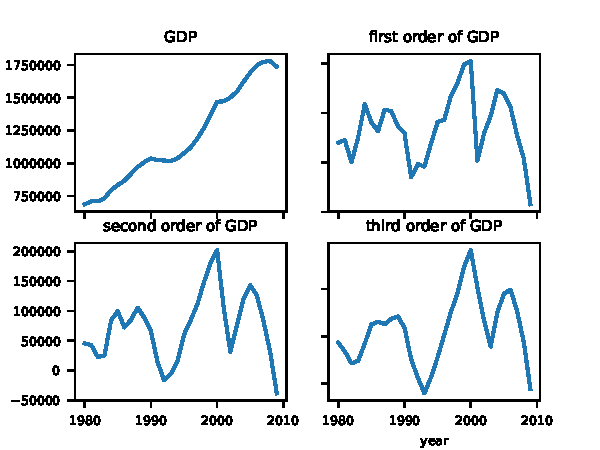
\includegraphics[width=0.5\linewidth]{fig/gdp_diff.pdf}
    \caption{GDP, first, second and third order difference of GDP}
    \label{fig: gdp_diff}
\end{figure}

    \begin{figure}[H] 
    \centering 
    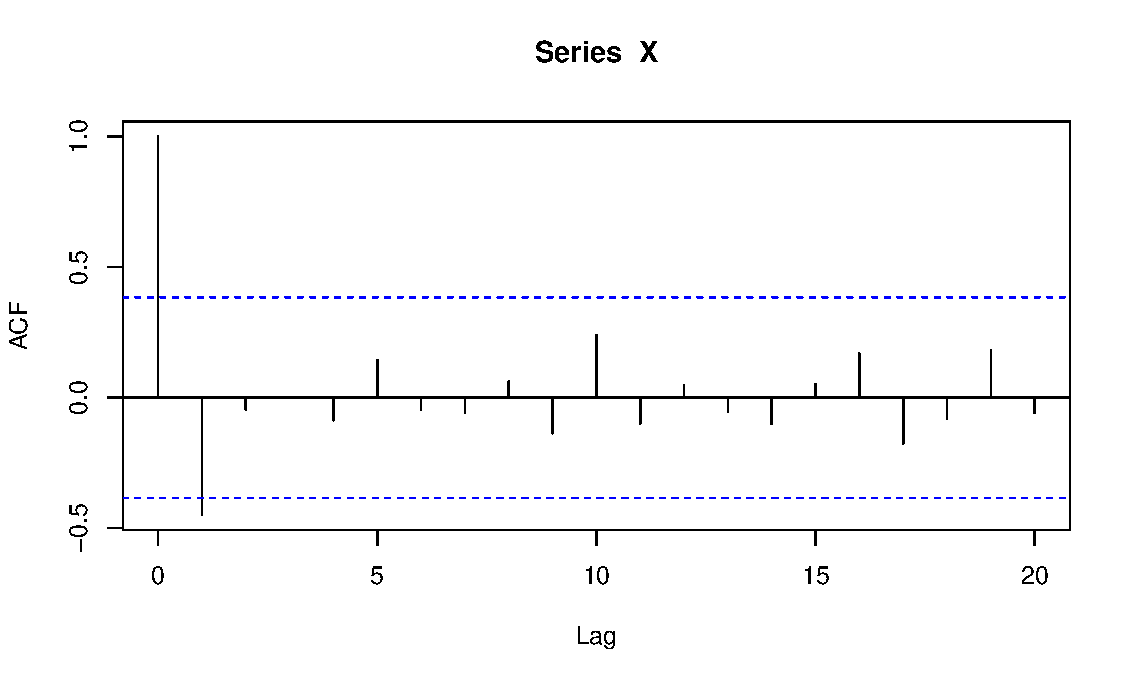
\includegraphics[width=0.5\linewidth]{fig/gdp_diff3_acf.pdf}
    \caption{Autocorrelation correlation function of first order difference of GDP}
    \label{fig: gdpacf}
    \end{figure}
    
    \begin{figure}[H] 
    \centering 
    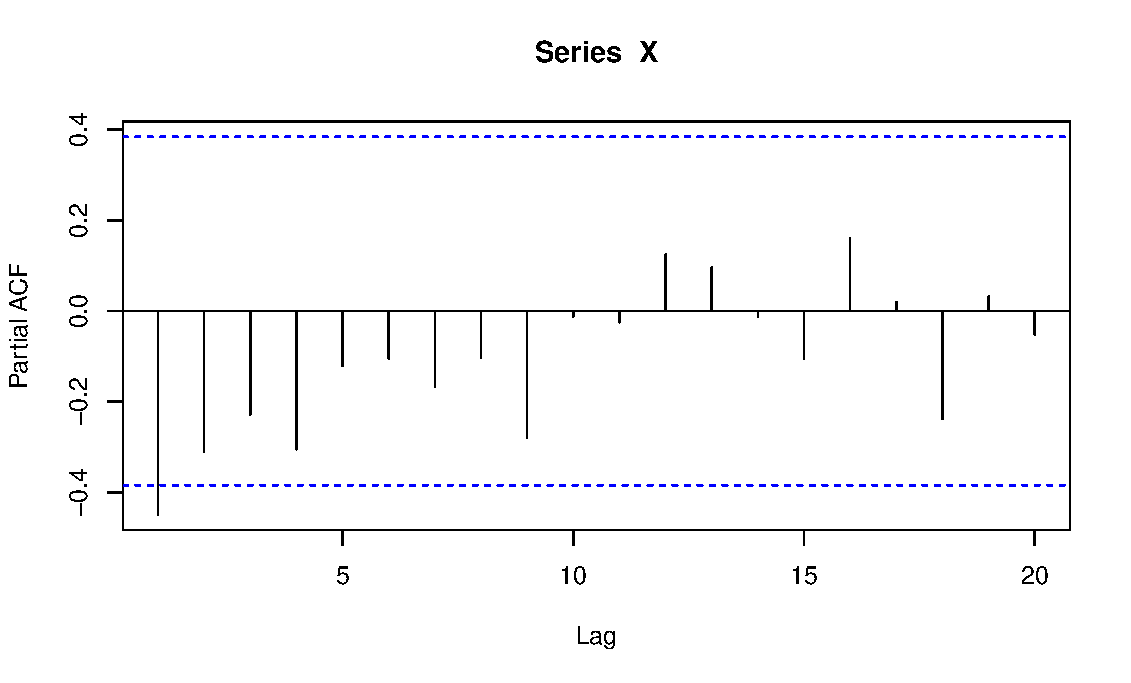
\includegraphics[width=0.5\linewidth]{fig/gdp_diff3_pacf.pdf}
    \caption{Partial autocorrelation function of first order difference of GDP}
    \label{fig: gdppacf}
    \end{figure}
    
            \begin{figure}[H] 
    \centering 
    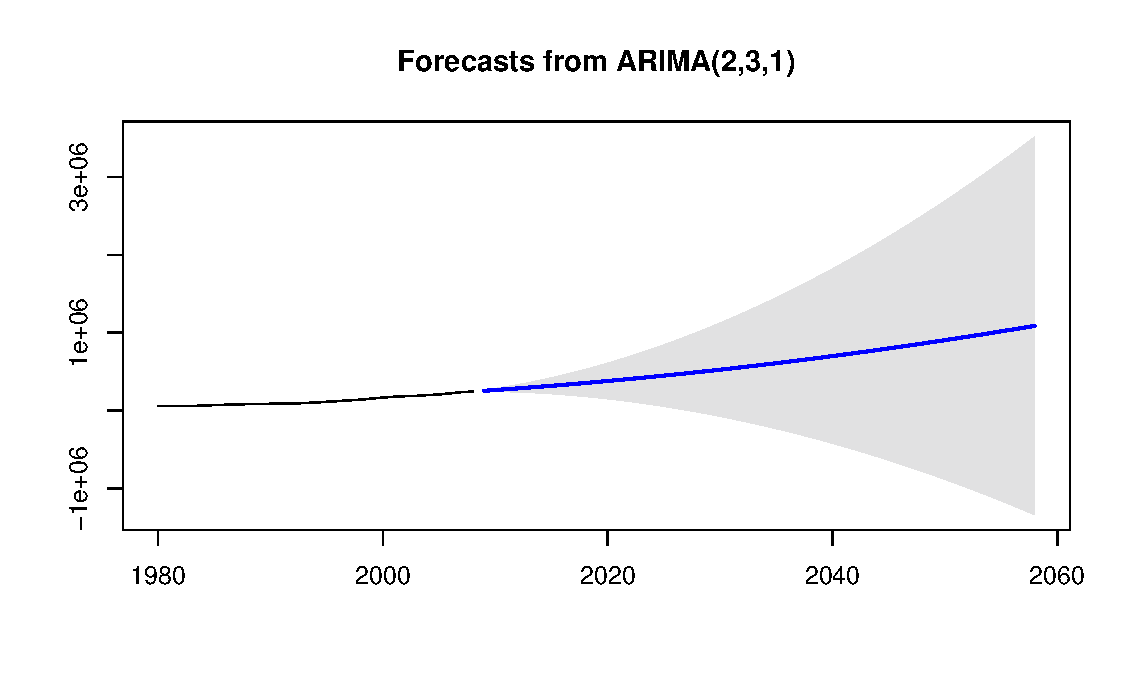
\includegraphics[width=0.5\linewidth]{fig/gdp_forecast.pdf}
    \caption{Forecast GDP with ARIMA (2, 3, 1)}
    \label{fig: gdpforecast}
    \end{figure}
    
    \item{Prediction of energy profile with predicted main factors}\par
    The prediction of the energy profile is shown in figure \ref{fig: energy profile prediction}. We can draw out the features in the figure during 2020$\sim$2050:
    \begin{itemize}
        \item California: proportion of petroleum will decrease slowly, while proportion of renewable energy will increase slowly.
        \item Arizona: proportion of natural gas will decrease, and nearly goes to zero. While proportion of nuclear energy increase quickly and exceed coal at the end of 2050.
        \item New Mexico: proportion of coal will transfer to natural gas, it is the only state that the proportion of natural gas keeps increasing.
        \item Texas: proportion of natural gas will fade away, will that of coal, natural gas  and renewable energy increase gradually.
    \end{itemize}
\end{enumerate}
\begin{figure}[H] 
    \centering 
    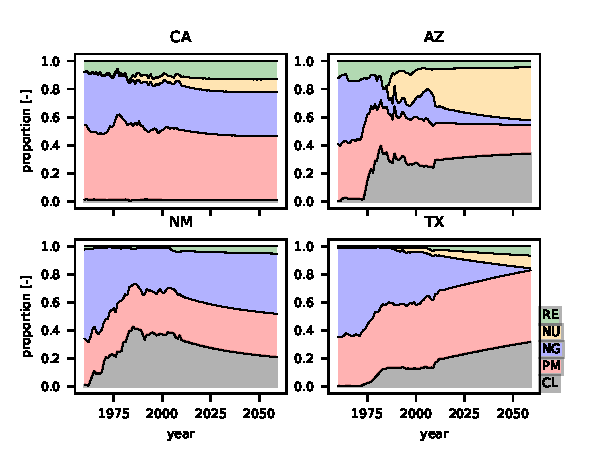
\includegraphics[width=0.5\linewidth]{fig/proportion_Prediction.pdf}
    \caption{Prediction of energy profile (profile before 2009 is regressed with real main factors, after 2009 is predicted based on multiple linear regression model before 2009 with predicted main factors)}
    \label{fig: energy profile prediction}
\end{figure}